% System model figure (compiled to EPS by make_figs.py:  pdflatex -> pdftops -eps)
\documentclass[border=1pt]{standalone}
\usepackage{tikz}
\usepackage{mathptmx}
\usetikzlibrary{arrows.meta,positioning,calc,decorations.pathreplacing,shapes.geometric}
\definecolor{cv}{HTML}{0072B2}
\definecolor{zoh}{HTML}{D55E00}
\definecolor{loi}{HTML}{009E73}
\definecolor{road}{HTML}{E9ECEF}
\definecolor{truck}{HTML}{6C757D}
\begin{document}
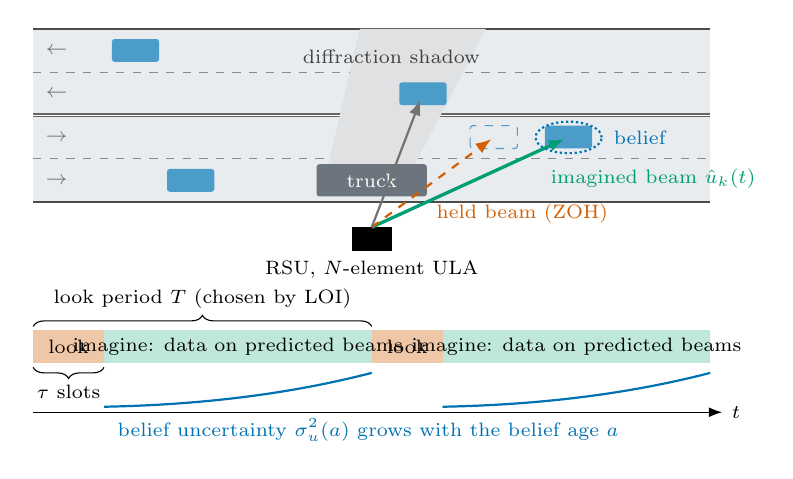
\begin{tikzpicture}[x=1cm,y=1cm,every node/.style={font=\scriptsize}]
% ---------------- scene ----------------
\fill[road] (0,0) rectangle (8.6,2.2);
\draw[thick,black!70] (0,0)--(8.6,0); \draw[thick,black!70] (0,2.2)--(8.6,2.2);
\draw[dashed,black!45] (0,0.55)--(8.6,0.55); \draw[double,black!60] (0,1.1)--(8.6,1.1);
\draw[dashed,black!45] (0,1.65)--(8.6,1.65);
\foreach \y/\a in {0.27/$\rightarrow$,0.82/$\rightarrow$,1.37/$\leftarrow$,1.92/$\leftarrow$}
  \node[black!55] at (0.3,\y) {\a};
% shadow region behind the truck (drawn first)
\fill[truck!22] (3.75,0.48)--(4.85,0.48)--(5.75,2.2)--(4.15,2.2)--cycle;
% vehicles
\fill[cv!70,rounded corners=1pt] (1.7,0.13) rectangle (2.3,0.42);
\draw[cv!70,dashed,rounded corners=1pt] (5.55,0.68) rectangle (6.15,0.97);
\fill[cv!70,rounded corners=1pt] (6.5,0.68) rectangle (7.1,0.97);
\fill[truck,rounded corners=1pt] (3.6,0.07) rectangle (5.0,0.48); \node[white] at (4.3,0.27) {truck};
\fill[cv!70,rounded corners=1pt] (4.65,1.23) rectangle (5.25,1.52);
\fill[cv!70,rounded corners=1pt] (1.0,1.78) rectangle (1.6,2.07);
% RSU
\draw[fill=black] (4.05,-0.62) rectangle (4.55,-0.32);
\node[below=0pt] at (4.3,-0.62) {RSU, $N$-element ULA};
% beams
\draw[loi,very thick,-{Latex[length=2mm]}] (4.3,-0.32)--(6.75,0.80);
\draw[zoh,thick,dashed,-{Latex[length=2mm]}] (4.3,-0.32)--(5.82,0.80);
\draw[black!55,thick,-{Latex[length=2mm]}] (4.3,-0.32)--(4.92,1.30);
\node[black!75] at (4.55,1.85) {diffraction shadow};
\draw[cv,densely dotted,thick] (6.8,0.82) ellipse (0.42 and 0.2);
\node[cv,anchor=west] at (7.25,0.82) {belief};
\node[zoh,anchor=west] at (5.0,-0.15) {held beam (ZOH)};
\node[loi,anchor=west] at (6.45,0.30) {imagined beam $\hat u_k(t)$};
% ---------------- timeline ----------------
\begin{scope}[yshift=-2.05cm]
\foreach \x in {0,4.3} {\fill[zoh!35] (\x,0) rectangle ++(0.9,0.42); \node at (\x+0.45,0.21) {look};}
\foreach \x in {0.9,5.2} {\fill[loi!25] (\x,0) rectangle ++(3.4,0.42); \node at (\x+1.7,0.21) {imagine: data on predicted beams};}
\draw[decorate,decoration={brace,amplitude=4pt,mirror}] (0,-0.05)--(0.9,-0.05) node[midway,below=3pt] {$\tau$ slots};
\draw[decorate,decoration={brace,amplitude=4pt}] (0,0.47)--(4.3,0.47) node[midway,above=3pt] {look period $T$ (chosen by LOI)};
\draw[-{Latex}] (0,-0.62)--(8.75,-0.62) node[right] {$t$};
\draw[cv,thick] (0.9,-0.55) .. controls (2.5,-0.52) and (3.6,-0.30) .. (4.3,-0.12);
\draw[cv,thick] (5.2,-0.55) .. controls (6.8,-0.52) and (7.9,-0.30) .. (8.6,-0.12);
\node[cv,anchor=west] at (0.95,-0.85) {belief uncertainty $\sigma_u^2(a)$ grows with the belief age $a$};
\end{scope}
\end{tikzpicture}
\end{document}
